\section{Proposta}

\subsection{A aplicação Price Search}
A aplicação PriceSearch foi pensado com o intuito de facilitar a pesquisa de preço de qualquer tipo de item existente no mercado, sejam eles eletrodomésticos, alimentos, utensílios, remédios, etc. Hoje em dia podemos encontrar diversos tipos de produtos em sites de grandes lojas, porém como existem várias cidades no Brasil que não possuem dessas grandes lojas, percebe-se que há uma grande dificuldade para saber em qual lugar tem tal item mais barato. Com isso, a ideia da aplicação é que as pessoas tenham acesso à um recurso para comparação de preço dos produtos dos estabelecimentos locais, a fim de ajudar as pessoas à economizar dinheiro. 

Outra ideia da aplicação é ajudar na busca de produtos, que antes não se sabia onde vendia. Com uma simples pesquisa, o usuário pode identificar facilmente o valor desse produto e onde encontrá-lo, através de um mapa que fornecerá a localização do estabelecimento contendo o seu endereço.

O intuito foi criar uma ferramenta simples, de fácil uso, e sendo ela multiplataformas, com o objetivo de agregar a quantidade máxima de usuários possíveis, para que todos possam usá-lo de maneira eficiente e rápida.

\subsection{Progressive web app}

O PWA é uma aplicação web que também se comporta como uma uma aplicação nativa, ele facilita o desenvolvimento de aplicações. Ele utiliza servisse workers, que são scripts que controlam o armazenamento de cache, fornecendo um melhor desempenho pois permite que os assetes e boa parte do front-and persista armazenado no dispositivo, isso faz com que em alguns casos seja possível utiliza-lo completamente off-line.

Mesmo sendo uma aplicação web, o PWA pode acessar todos os recursos do celular, como câmera, GPS e contatos, assim facilitando a vida do usuário.

Diferente dos aplicativos que necessitam que ele seja baixado de uma app store, a única coisa que o usuário precisa fazer e entrar no site e caso goste ele pode salvar a aplicação web no seu celular, como se fosse um app mobile.


\subsection{Diagrama de Blocos}

 Donec accumsan orci luctus dolor sagittis viverra. Praesent vel leo at tellus vestibulum pulvinar. Duis laoreet sapien diam. Quisque condimentum tincidunt imperdiet. Ut vehicula mattis nisi lobortis viverra. Nullam id lorem ante. Maecenas sodales neque purus, ut eleifend ipsum consectetur non. In vehicula nisl augue, eu tempor enim vulputate vitae.
 
\begin{figure}[!htb]
\centering
\caption{Imagem de exemplo.}
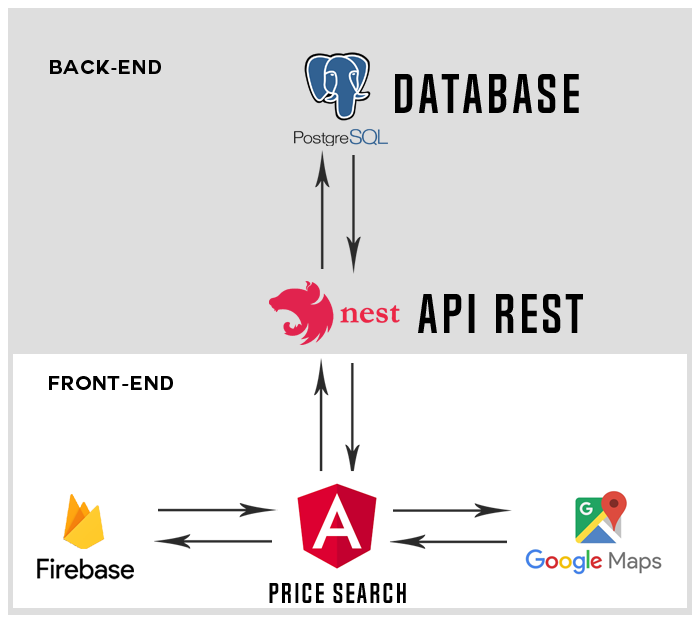
\includegraphics[width=\linewidth]{figuras/diagrama_de_blocos.png}
\end{figure}
 
 Vivamus ullamcorper metus et felis tincidunt consequat. Cras eu augue faucibus, viverra odio id, placerat nibh. Duis et efficitur ex. Donec tincidunt suscipit lacus, id interdum sem posuere vel. Pellentesque habitant morbi tristique senectus et netus et malesuada fames ac turpis egestas. Nullam tristique dictum congue. Donec ut neque non magna faucibus tempor quis id dolor. 

\subsection{Modelo de Dados}
 
 Lorem ipsum dolor sit amet, consectetur adipiscing elit. Suspendisse eros ligula, semper sit amet viverra eget, bibendum quis massa. Nullam urna enim, euismod non sapien vel, ornare ullamcorper sem. Proin faucibus, magna in pharetra efficitur, augue nibh volutpat lorem, eu porttitor nulla eros in nibh. Etiam nec dui vitae ligula tincidunt accumsan.
 
\begin{figure}[!htb]
\centering
\caption{Imagem de exemplo.}
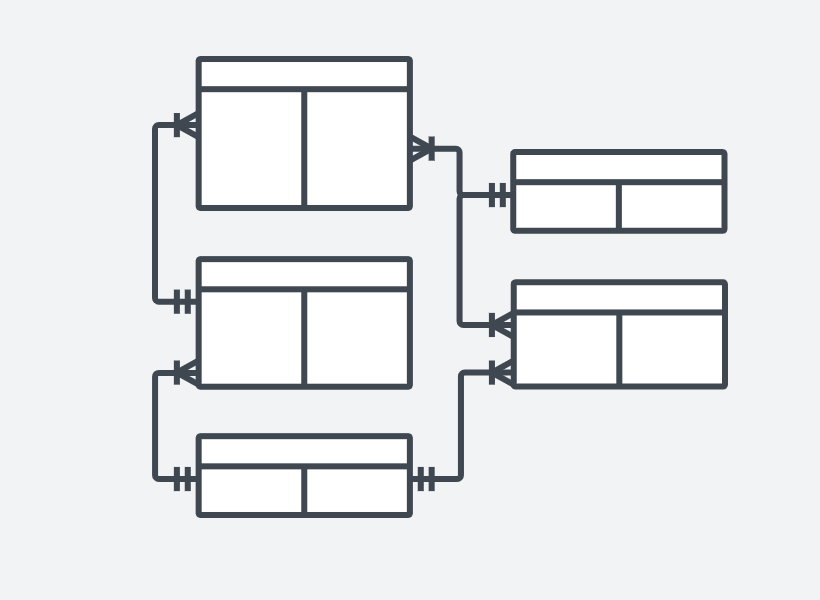
\includegraphics[width=\linewidth]{figuras/mer.png}
\end{figure}
 
 Cras eu nisi volutpat leo efficitur sagittis a vehicula orci. Integer sed erat vel purus ullamcorper faucibus at in tortor. Donec laoreet faucibus lacus, eget cursus quam lacinia at. Aliquam interdum lorem eu nulla laoreet, sed blandit nisi rhoncus. Sed vitae consectetur massa, ut scelerisque urna. Maecenas sed condimentum quam, in dignissim lectus. 
 
 \subsection{Casos de Uso}
O diagrama de casos de uso da aplicação ilustra as ações de um usuário, que terá acesso às funções listadas, conforme a figura abaixo:

\begin{figure}[!htb]
\centering
\caption{Diagrama de Casos de Uso Price Search.}
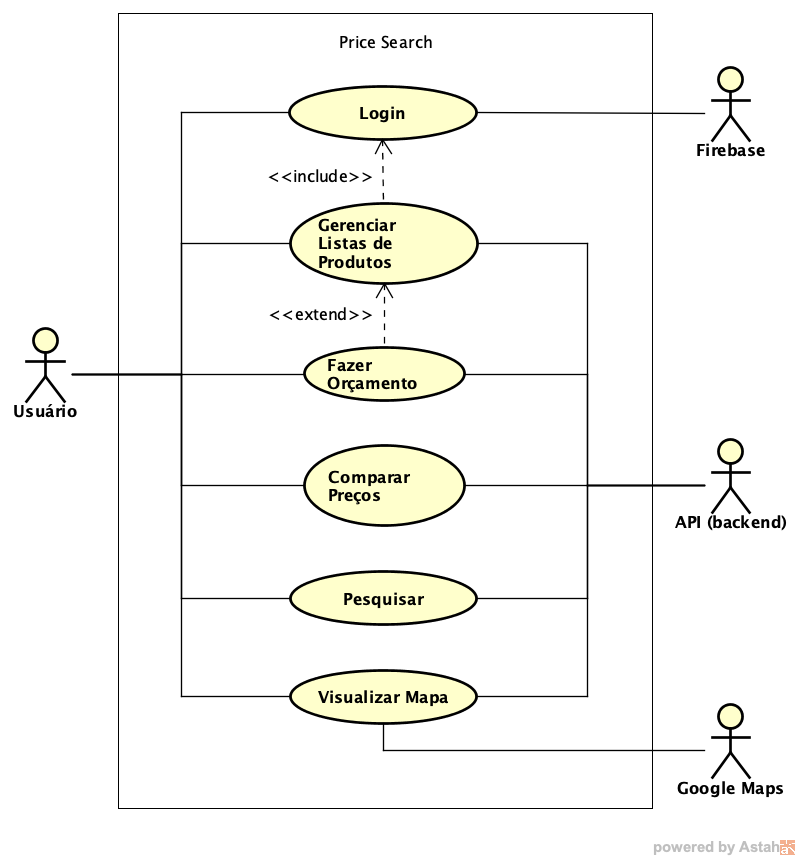
\includegraphics[width=\linewidth]{figuras/DiagramaCasosUsoPriceSearch.png}
{\footnotesize Fonte: Elaborado pelo autor.}
\end{figure}

\subsubsection{Caso de Uso 01: Login usuário}

O usuário inicia o login utilizando uma conta existente da Google, não sendo necessário preenchimento de nenhum tipo de dados. Feito isso, o assistente irá validar os dados do mesmo e o login será efetuado. Feito isso, nossa aplicação utilizará do ‘token’ fornecido pela conta do Google, para que possa ser salvo em nosso banco de dados para a sincronização das informações do usuário.

\begin{figure}[!htb]
\centering
\caption{Imagem de exemplo.}
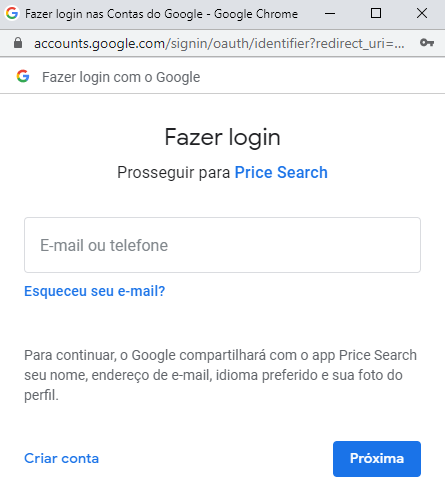
\includegraphics[width=\linewidth]{figuras/tela-login.png}
\end{figure}

\subsubsection{Caso de Uso 02: Pesquisar}

A barra de pesquisa se encontra no topo da página, junto dela também existe um botão de menu para mostrar todas as abas do aplicativo. A pesquisa será feita através dos nome de produtos, então o usuário poderá pesquisar por qualquer item, desde que o mesmo esteja no banco de dados, e o sistema irá retornar todos os itens que tem o mesmo nome. (perguntar se adiciona filtro).

\begin{figure}[!htb]
\centering
\caption{Imagem de exemplo.}
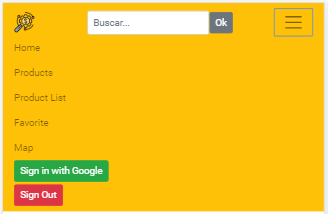
\includegraphics[width=\linewidth]{figuras/tela-menu.png}
\end{figure}

\subsubsection{Caso de Uso 03: Gerenciar Lista de Compra}

O usuário poderá criar várias listas de compra como se fosse um carrinho de compras. Ao criar uma lista, o usuário poderá escolher um nome para ela; bem como escolher quais itens serão adicionados, e removê-los a qualquer momento; ou mesmo renomear a lista ou exclui-lá.

\begin{figure}[!htb]
\centering
\caption{Tela onde mostram todos os produtos disponíveis.}
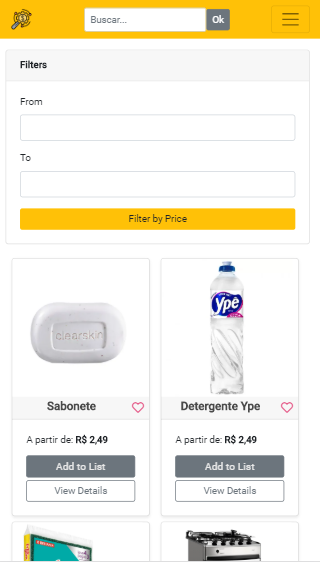
\includegraphics[width=\linewidth]{figuras/tela_lista_produtos.png}
\end{figure}

\subsubsection{Caso de Uso 04: Comparar Preços}

O usuário poderá comparar preços de um produto em diferentes estabelecimentos, e através do aplicativo descobrir em qual estabelecimento ele pode encontrar o melhor preço do produto que deseja.

\begin{figure}[!htb]
\centering
\caption{Imagem de exemplo.}

\includegraphics[width=\linewidth]{figuras/placeholder.jpg}
\end{figure}

\subsubsection{Caso de Uso 05: Fazer Orçamento}

O usuário poderá criar listas de compra e ao fazer isso ele poderá realizar o orçamento delas nos estabelecimentos desejados, assim podendo orçar todo a compra de uma vez, e descobrir onde ela ficara mais barata.

\begin{figure}[!htb]
\centering
\caption{Imagem de exemplo.}

\includegraphics[width=\linewidth]{figuras/placeholder.jpg}
\end{figure}

\subsubsection{Caso de Uso 06: Visualizar Mapa}

O usuário terá acesso à um mapa que contém a localização de todos os estabelecimentos locais cadastrados. Ao clicar nos estabelecimentos mostrados no mapa, irá ser fornecido informações sobre ele, como nome e endereço.


\begin{figure}[!htb]
\centering
\caption{Imagem de exemplo.}
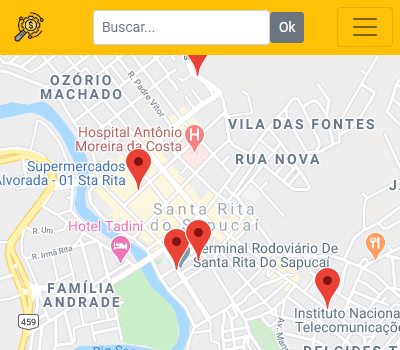
\includegraphics[width=\linewidth]{figuras/tela_mapa.png}
\end{figure}
